\documentclass{article}
\usepackage[utf8]{inputenc}
\usepackage[backend=biber]{biblatex}
\usepackage{amssymb}
\usepackage{amsmath}
\usepackage{dsfont}
\addbibresource{bib.bib}
\setlength{\parindent}{0em}
\bibliography{bib}
\setlength{\parskip}{6pt}
\usepackage[margin=1.0in]{geometry}
\usepackage{graphicx}
\usepackage{caption}
\usepackage{subcaption}
\usepackage{wrapfig}
\usepackage{url}

\title{Intro to deep learning with PyTorch}
\author{Miguel A. Saavedra-Ruiz}
\date{May 2020}
\linespread{1.0}

\nocite{*}


\begin{document}

\maketitle

\section*{Transfer Style}

Convolutional neural networks have a lot of applications. These are not only used for image classification but to construct images as well with the information in the filters. The representation of new images based on CNNs is called style transfer and deep dream Fig. \ref{fig:f1}. Style transfer compose images based on CNN layer activation and extracted features. This technique allows to apply the style of one image to another image.

\begin{figure}[ht]
    \centering
    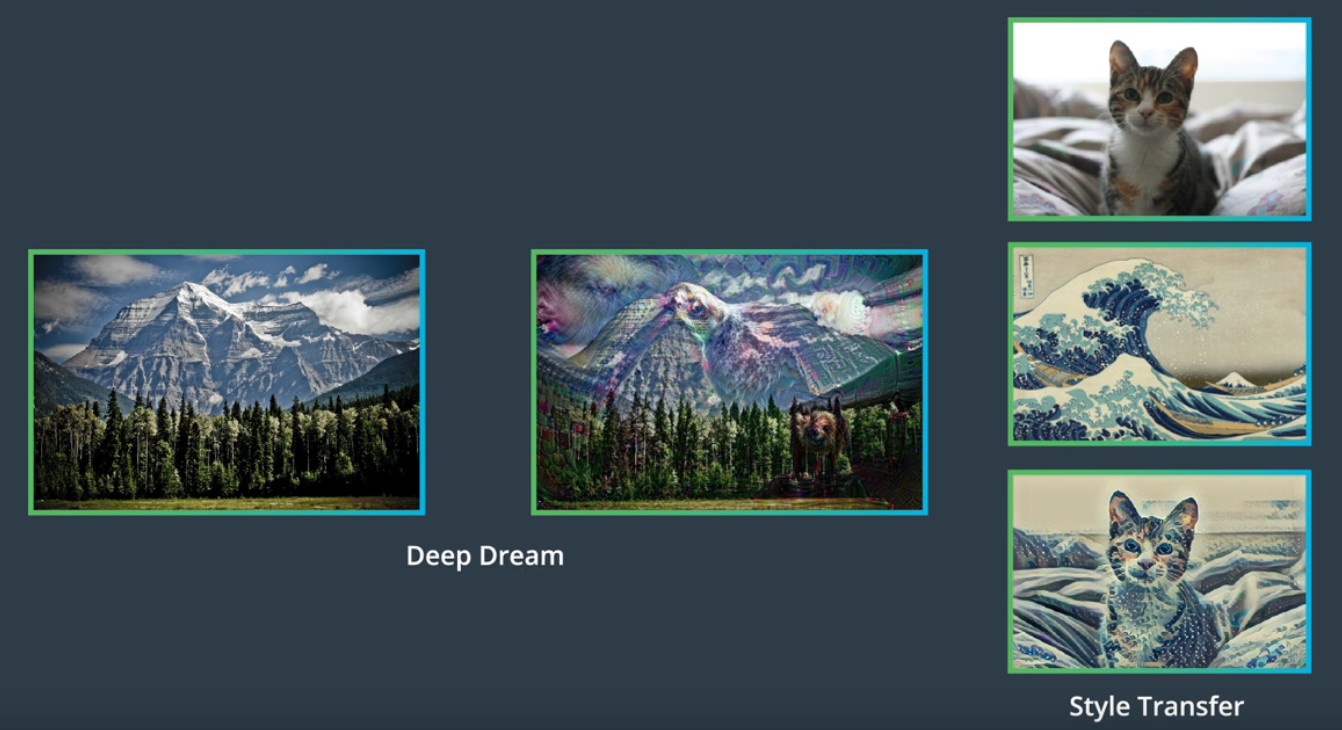
\includegraphics[width=0.8\textwidth,height=0.8\textheight,keepaspectratio]{images/style_transfer.png}
    \captionsetup{justification=centering}
    \caption{Features in an image}
    \label{fig:f1}
\end{figure}

This technique works by separating the content from the style on an image and merge it with another image.

To understand transfer style it is important to understand the concept of \textbf{content} and \textbf{style} and how this is related to CNNs. When a CNN is trained to classify images, its convolutional layers learn to extract more and more complex features from a given image. Intermittently, max pooling layers will discard detailed spatial information, information that's increasingly irrelevant to the task of classification. The effect of this is that as the network goes deeper, the input image is transformed into feature maps that increasingly care about the \textbf{content} of the image rather than any detail about the texture and color of pixels. Later layers of a network are even sometimes referred to as a content representation of an image Fig. \ref{fig:f2}. Therefore, a normal trained CNN already has learned how to extract content of an image.

\begin{figure}[ht]
    \centering
    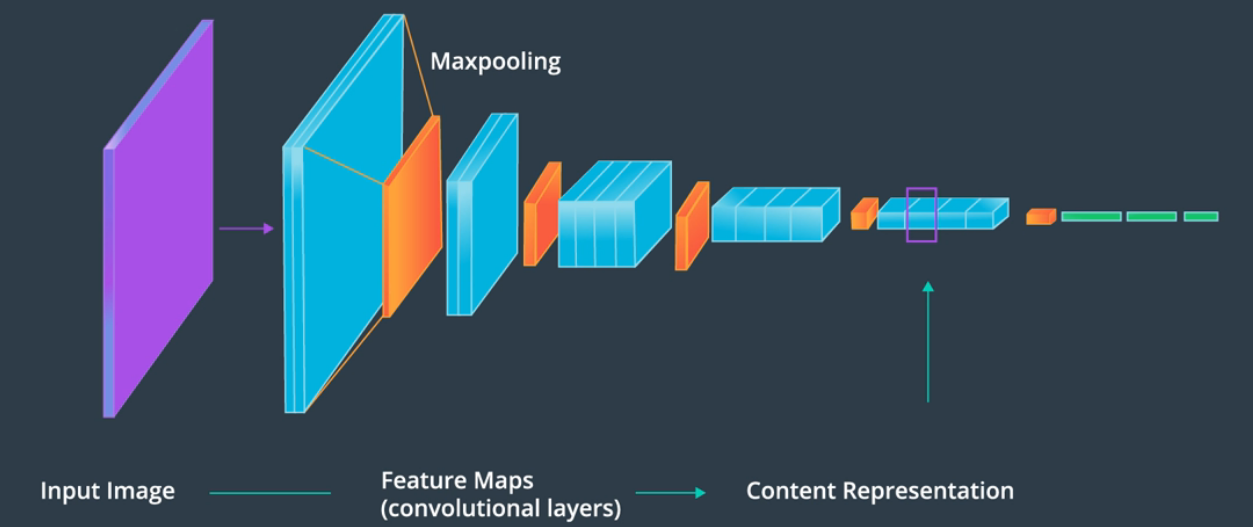
\includegraphics[width=0.8\textwidth,height=0.8\textheight,keepaspectratio]{images/content.png}
    \captionsetup{justification=centering}
    \caption{Extracting content with a CNN}
    \label{fig:f2}
\end{figure}

To represent the \textbf{style} of an image a feature space designed to capture texture and color information needs to be used. A feature space designed to capture texture and color information is employed. This space essentially looks at spatial correlations within a layer of a network. A correlation is a measure of the relationship between two or more variables.

In the context of CNNs, For each feature map it is possible to measure how strongly each detected feature is relate to the other feature maps in that layer. Check which colors and shapes in a set of feature maps are related and which are not. Imagine that a mini-feature map is detected in the first convolutional layer with similar pink edge features Fig. \ref{fig:f3}. If there are common colors and shapes among the feature maps, then this can be thought of as part of that image's style. Hence, the similarities and differences between features in a layer should bring some information about the texture and color information found in an image.


\begin{figure}[ht]
    \centering
    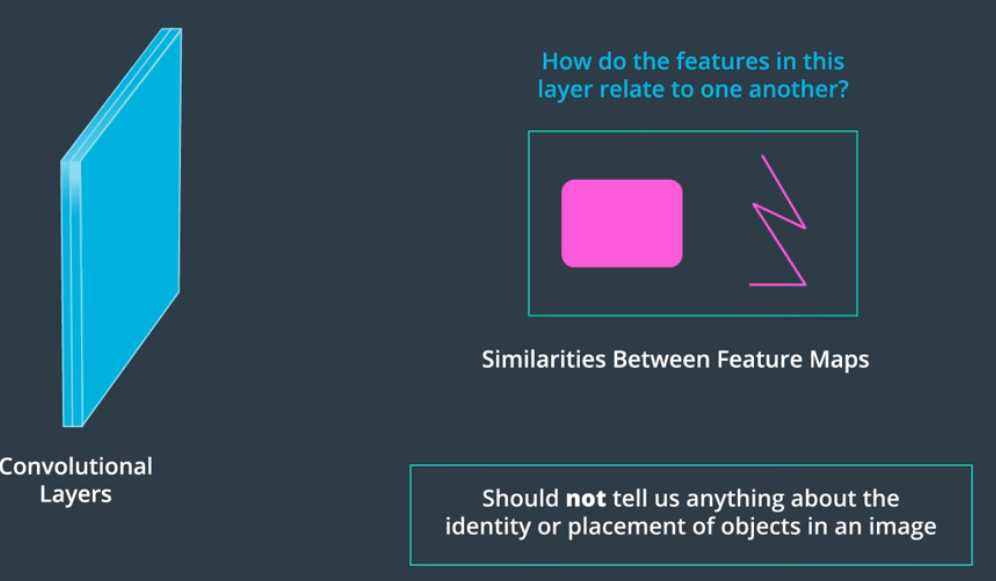
\includegraphics[width=0.7\textwidth,height=0.7\textheight,keepaspectratio]{images/style.png}
    \captionsetup{justification=centering}
    \caption{Extracting style of an image with a CNN}
    \label{fig:f3}
\end{figure}

Style transfer works by looking at two different images. These images are oftenly called the style image and the content image. Using a trained CNN, style transfer finds the style of one image and the content of the other. Finally, it tries to merge the two to create a new third image. The objects and their arrangement are taken from the content image, and the colors and textures are taken from the style image.

Fig. \ref{fig:f2} shows the VGG-19 (19 convolutional layers) architecture which is used to do style transfer. To extract the content of an image first this is passed through the network and the features of the convolutional layer with the purple rectangle is obtained (Fig. \ref{fig:f2}). Then, the style image is passed through the network and the style representations are extracted from the layers in Fig. \ref{fig:f4}

\begin{figure}[ht]
    \centering
    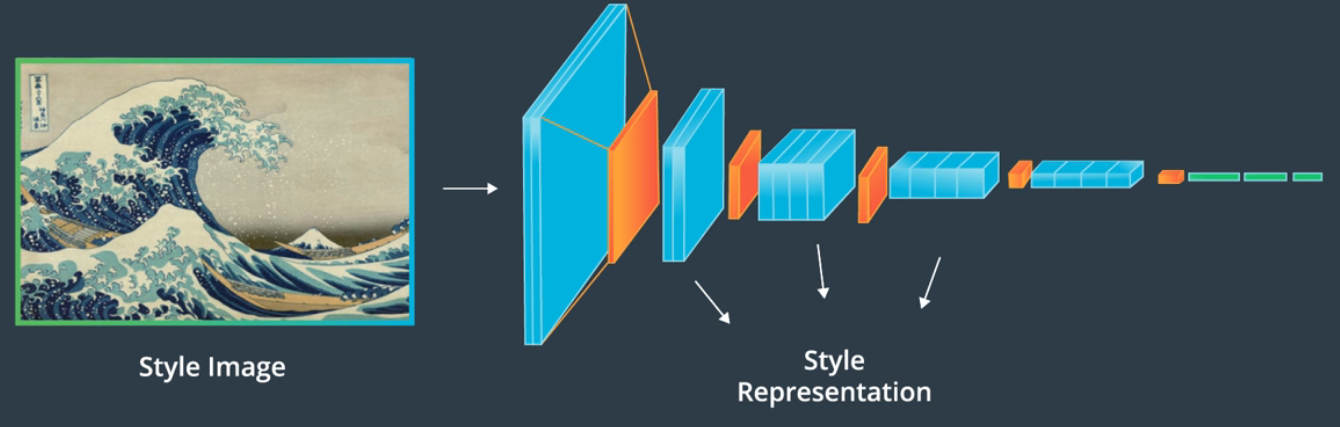
\includegraphics[width=0.7\textwidth,height=0.7\textheight,keepaspectratio]{images/style_cnn.png}
    \captionsetup{justification=centering}
    \caption{Style representation in a CNN}
    \label{fig:f4}
\end{figure}

Finally both the content and style representations are used to create the target image (new image representation). While the target image is being formed, the target image content representation is compared with the content image representation and these must be very similar Fig. \ref{fig:f5}. These two representations should be close to the same even as the target image change its style.

\begin{figure}[ht]
    \centering
    
\includegraphics[width=0.5\textwidth,height=0.5\textheight,keepaspectratio]{images/content_target.png}
    \captionsetup{justification=centering}
    \caption{Similarity between content and target}
    \label{fig:f5}
\end{figure}

To formalize the last thing said, it is necessary to formalize a content loss that calculates the difference between the content and target image representations. The content representation from the content image will be called \(\boldsymbol{C_c}\) and the one from the target image \(\boldsymbol{T_c}\). In this case the loss content will be defined as the mean squared difference between the two representations Eq. \eqref{eq:1}. This loss function measures how far away these two representations are from one another. As the algorithm aims to create the best target image the objective is to minimize this loss.

\begin{equation}
L_{content} = \frac{1}{2} \sum(T_c - C_c)^2
\label{eq:1}
\end{equation}

In this occasion the CNNs is not being trained to classified an image but to change only the target image, updating its appearance until it's content representation matches that of the content image. \textbf{The CNN is used to extract features and minimize the loss content and style loss.}

For the style representation of the image, recall that it relies on looking correlations between the features in individual layers of the VGG-19 network (CNN). Similarities will include the general colors and textures found in that layer. As shown in Fig. \ref{fig:f4}, the style representations are extracted from certain convolutional layers and as long as the network starts going deeper, it is possible to obtain a multi-scale style representation of the input image.

The correlations in each layer of the CNN are given by something called \textbf{Gram matrix}. This matrix is the result of a couple of operations which will be explained next. First of all image a four by four image, which is convolve with eight different image filters to create a convolutional layer. This layer will be four by four in height and width, and eight in depth. Thinking about the style representation for this layer, it is possible to say that this layer has eight feature maps where is possible to find the relationships between Fig. \ref{fig:f6}.

\begin{figure}[ht]
    \centering
    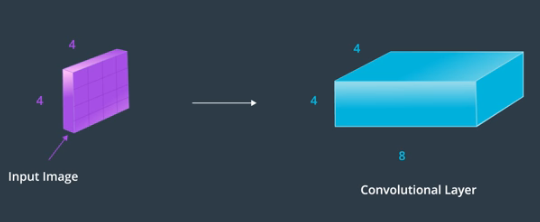
\includegraphics[width=0.5\textwidth,height=0.5\textheight,keepaspectratio]{images/conv_layer.png}
    \captionsetup{justification=centering}
    \caption{Generating a feature map for the Gram matrix}
    \label{fig:f6}
\end{figure}

The next step in calculating the Gram matrix, will be to vectorize (flattening) the values in one convolutional layer. This process is repeated with each layer of the feature map to finally obtain a 8x16 matrix representing the feature map as a matrix Fig. \ref{fig:f7}.

\begin{figure}[ht]
    \centering
    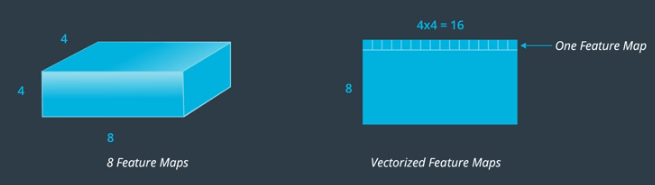
\includegraphics[width=0.5\textwidth,height=0.5\textheight,keepaspectratio]{images/f_map.png}
    \captionsetup{justification=centering}
    \caption{Feature map as a matrix}
    \label{fig:f7}
\end{figure}

The final step is to multiply the new 8x16 matrix by its transpose. Essentially, multiplying the features in each map to get the gram matrix. This operation treats each value in the feature map as an individual sample, unrelated in space to other values. The resultant Gram matrix contains non-localized information about the layer. Non-localized information, is information that would still be there even if an image was shuffled around in space. For example, even if the content of a filtered image is not identifiable, it is possible to see prominent colors and textures of the style. Finally, The result of the operation is the square eight by eight Gram matrix, whose values indicate the similarities between the the layers Fig. \ref{fig:f8}.

\begin{figure}[ht]
    \centering
    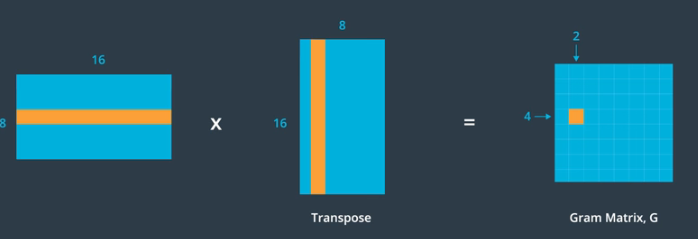
\includegraphics[width=0.6\textwidth,height=0.6\textheight,keepaspectratio]{images/gram.png}
    \captionsetup{justification=centering}
    \caption{The Gram matrix}
    \label{fig:f8}
\end{figure}

It is important to mention that the dimensions of this matrix are related only to the number of feature maps in the convolutional layer, it doesn't depend on the dimensions of the input image.

To calculate the style loss between a target and style image, it is necessary to find the mean squared distance between the style and target image gram matrices, all five pairs that are computed at each layer in the predefined list in VGG-19 Fig. \ref{fig:f4}. The five pairs are extracted from the feature maps shown in Fig. \ref{fig:f9}. conv1\_1 corresponds to the first feature map, conv2\_1 is the third convolution and so one. Notice that only the specified ones are the feature maps used to extract the style.

\begin{figure}[ht]
    \centering
    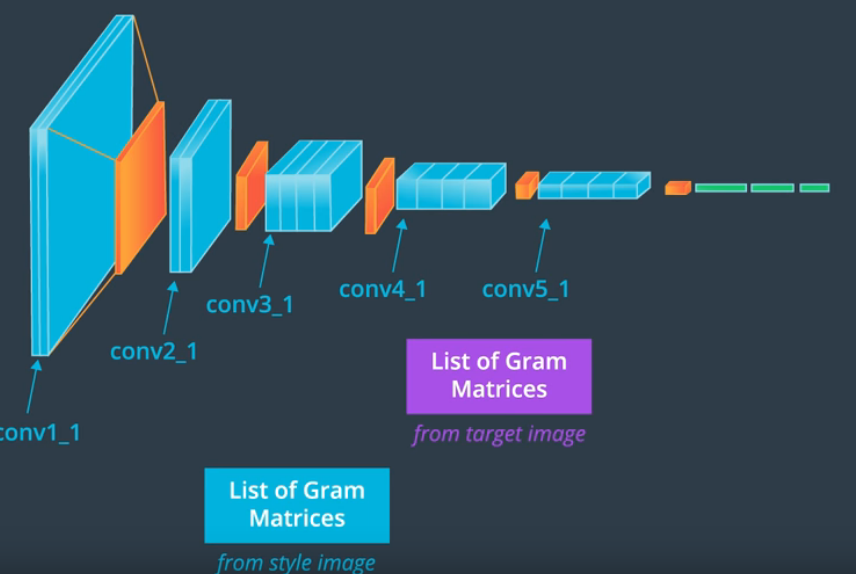
\includegraphics[width=0.6\textwidth,height=0.6\textheight,keepaspectratio]{images/extracting_style.png}
    \captionsetup{justification=centering}
    \caption{Extracting style from VGG-19}
    \label{fig:f9}
\end{figure}

The lists for the Style image in name \(\boldsymbol{S_s}\) and the one from the target image \(\boldsymbol{T_s}\). The Eq. \eqref{eq:2} shows the loss function for the style, where A is a constant that accounts for the number of values in each layer and \(W_i\) are the style weights that are specified by the user. The style weights are values that will give more or less weight to the calculated style loss at each of the five layers, thereby changing how much effect each layer style representation will have on the final target image.

\begin{equation}
L_{style} = a \sum_i w_i (S_{s,i} - T_{s,i})^2
\label{eq:2}
\end{equation}

Only the target image's style representations will be changing while minimizing the loss over some number of iterations.

Finally, the total loss is defined as the sum of the content loss and the target loss Eq. \eqref{eq:3}. This loss can be used to apply backpropagation and iteratively changing the target image to match the desired content and style.

\begin{equation}
L_{total} = \frac{1}{2} \sum(T_c - C_c)^2 + a \sum_i w_i (S_{s,i} - T_{s,i})^2
\label{eq:3}
\end{equation}

One detail about the total style transfer loss is that the function has different values for both content and style loss. Because they're calculated differently, these values will be pretty different, and the idea is that the target image take both into account fairly equally.

To solve this, it's necessary to apply constant weights, alpha and beta, to the content and style losses, such that the total loss reflects an equal balance. In practice, this means multiplying the style loss by a much larger weight value than the content loss Eq. \eqref{eq:4}. This will often be seen expressed as a ratio of the content and style weights, \(\frac{\alpha}{\beta}\). \(\alpha\) is frequently called content weight and \(\beta\) style weight.

\begin{equation}
L_{total} = \alpha (\frac{1}{2} \sum(T_c - C_c)^2) + \beta (a \sum_i w_i (S_{s,i} - T_{s,i})^2)
\label{eq:4}
\end{equation}

In general, the smaller the alpha-beta ratio, the more stylistic effect the target image will be. In the Fig. \ref{fig:f10} it is possible to see the effect of this ratio.

\begin{figure}[ht]
    \centering
    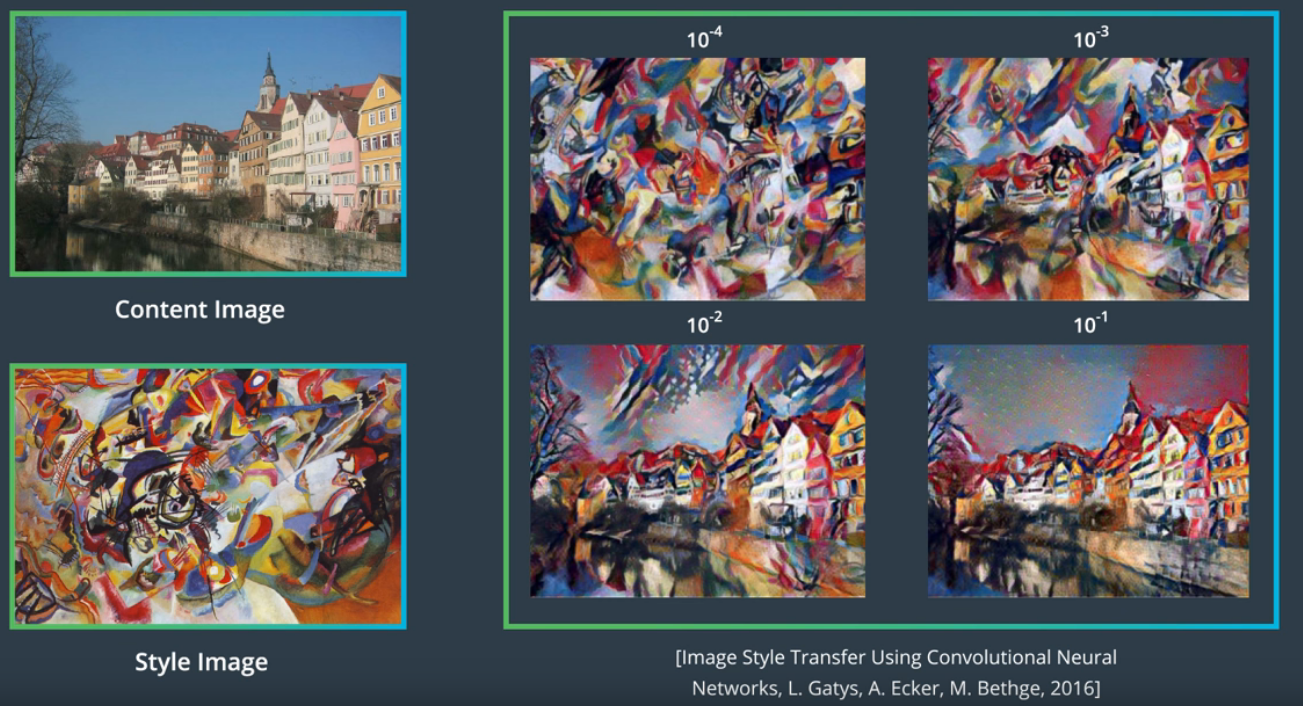
\includegraphics[width=0.55\textwidth,height=0.55\textheight,keepaspectratio]{images/beta.png}
    \captionsetup{justification=centering}
    \caption{The effect of the alpha-beta ratio}
    \label{fig:f10}
\end{figure}

It is important to mention again that the only thing that will change it the network is the target image. The weights of the network will not be touched at all. This variations in the target image is accomplished through the loss function.

A complete implementation of style transfer can be seen in Style\_Transfer.ipynb

\printbibliography


\end{document}
